\documentclass{article}
\usepackage{graphicx} % Required for inserting images
\usepackage{fancyhdr}
\cfoot{\thepage}
\lhead{\thepage}
\pagestyle{fancy}
\title{
    \vspace{2in}
    \textbf{Final Project}\\
    \vspace{2in}
}
\author{Parsa Arabshahi }
\date{Bahman 1402}
\begin{document}
\begin{titlepage}
\maketitle
\end{titlepage}
\newpage
\fancyhead[R]{\textbf{Table Of Contents}}
\tableofcontents
\newpage
\section{Git and Github:}
I created a new repository called FinalProject and i made sure that i had checked create a readme file.\\
For the automatic latex building i created \textit{.github} folder and in that i put \textit{workflows} folder. then i copied main.yml from \textit{CW1402Final} and pasted in it.\\
with each tags i commit (using git tag) and pushing, github automatically make the pdf for it.
\fancyhead[R]{}
\section{Exploration Tasks}
\subsection{Vim Advanced Features}
\subsubsection{g commands}
like gi. It can switch to insert and go to the last insertion you did or ga can print the ascii value of the character in decimal, hexadecimal or octal.
\subsubsection{Inserting and Deleting using CTRL}
like CTRL+a. It can insert the last thing you inserted or CTRL+w can delete the word under the cursor and more.
\subsubsection{Completion in Insert Mode}
CTRL+x CTRL+y : Scroll up\\
CTRL+x CTRL+e : Scroll down\\
CTRL+x s - Complete with spelling suggestions\\
...
\subsection{Memory profiling}
\subsubsection{Memory Leak}
Memory leaks can reduce system performance by reducing available memory.\\
It can cause when you forget to free the allocated memory.\\
Memory leaks can be very harmful in servers which never terminate.
\subsubsection{Memory profilers}
Valgrind tools can detect memory management and threading bugs. it provides a number of debugging and profiling tools which avoids memory leaking, and makes your program much faster.
\subsection{GNU/Linux Bash Scripting}
\subsubsection{fzf}
The difference between exact search and fuzzy searching is in fuzzy searching you can find approximate results which you may not know the exact spelling of the content but it can be found with fuzzy searching.\\
The command \texttt{ls | fzf} lists the file in the current directory using the ls command and pipes the output to fzf which allows you to search and select items from the list.
\subsubsection{Using fzf to find your favorite PDF}
\begin{enumerate}
    \item fd -e pdf /path/to/file
    \item -type f -name "filename" \texttt{|} fzf
\end{enumerate}
\subsubsection{Opening the file using Zathura}
zathura /path/to/file \$open filename
\section{Git and FOSS}
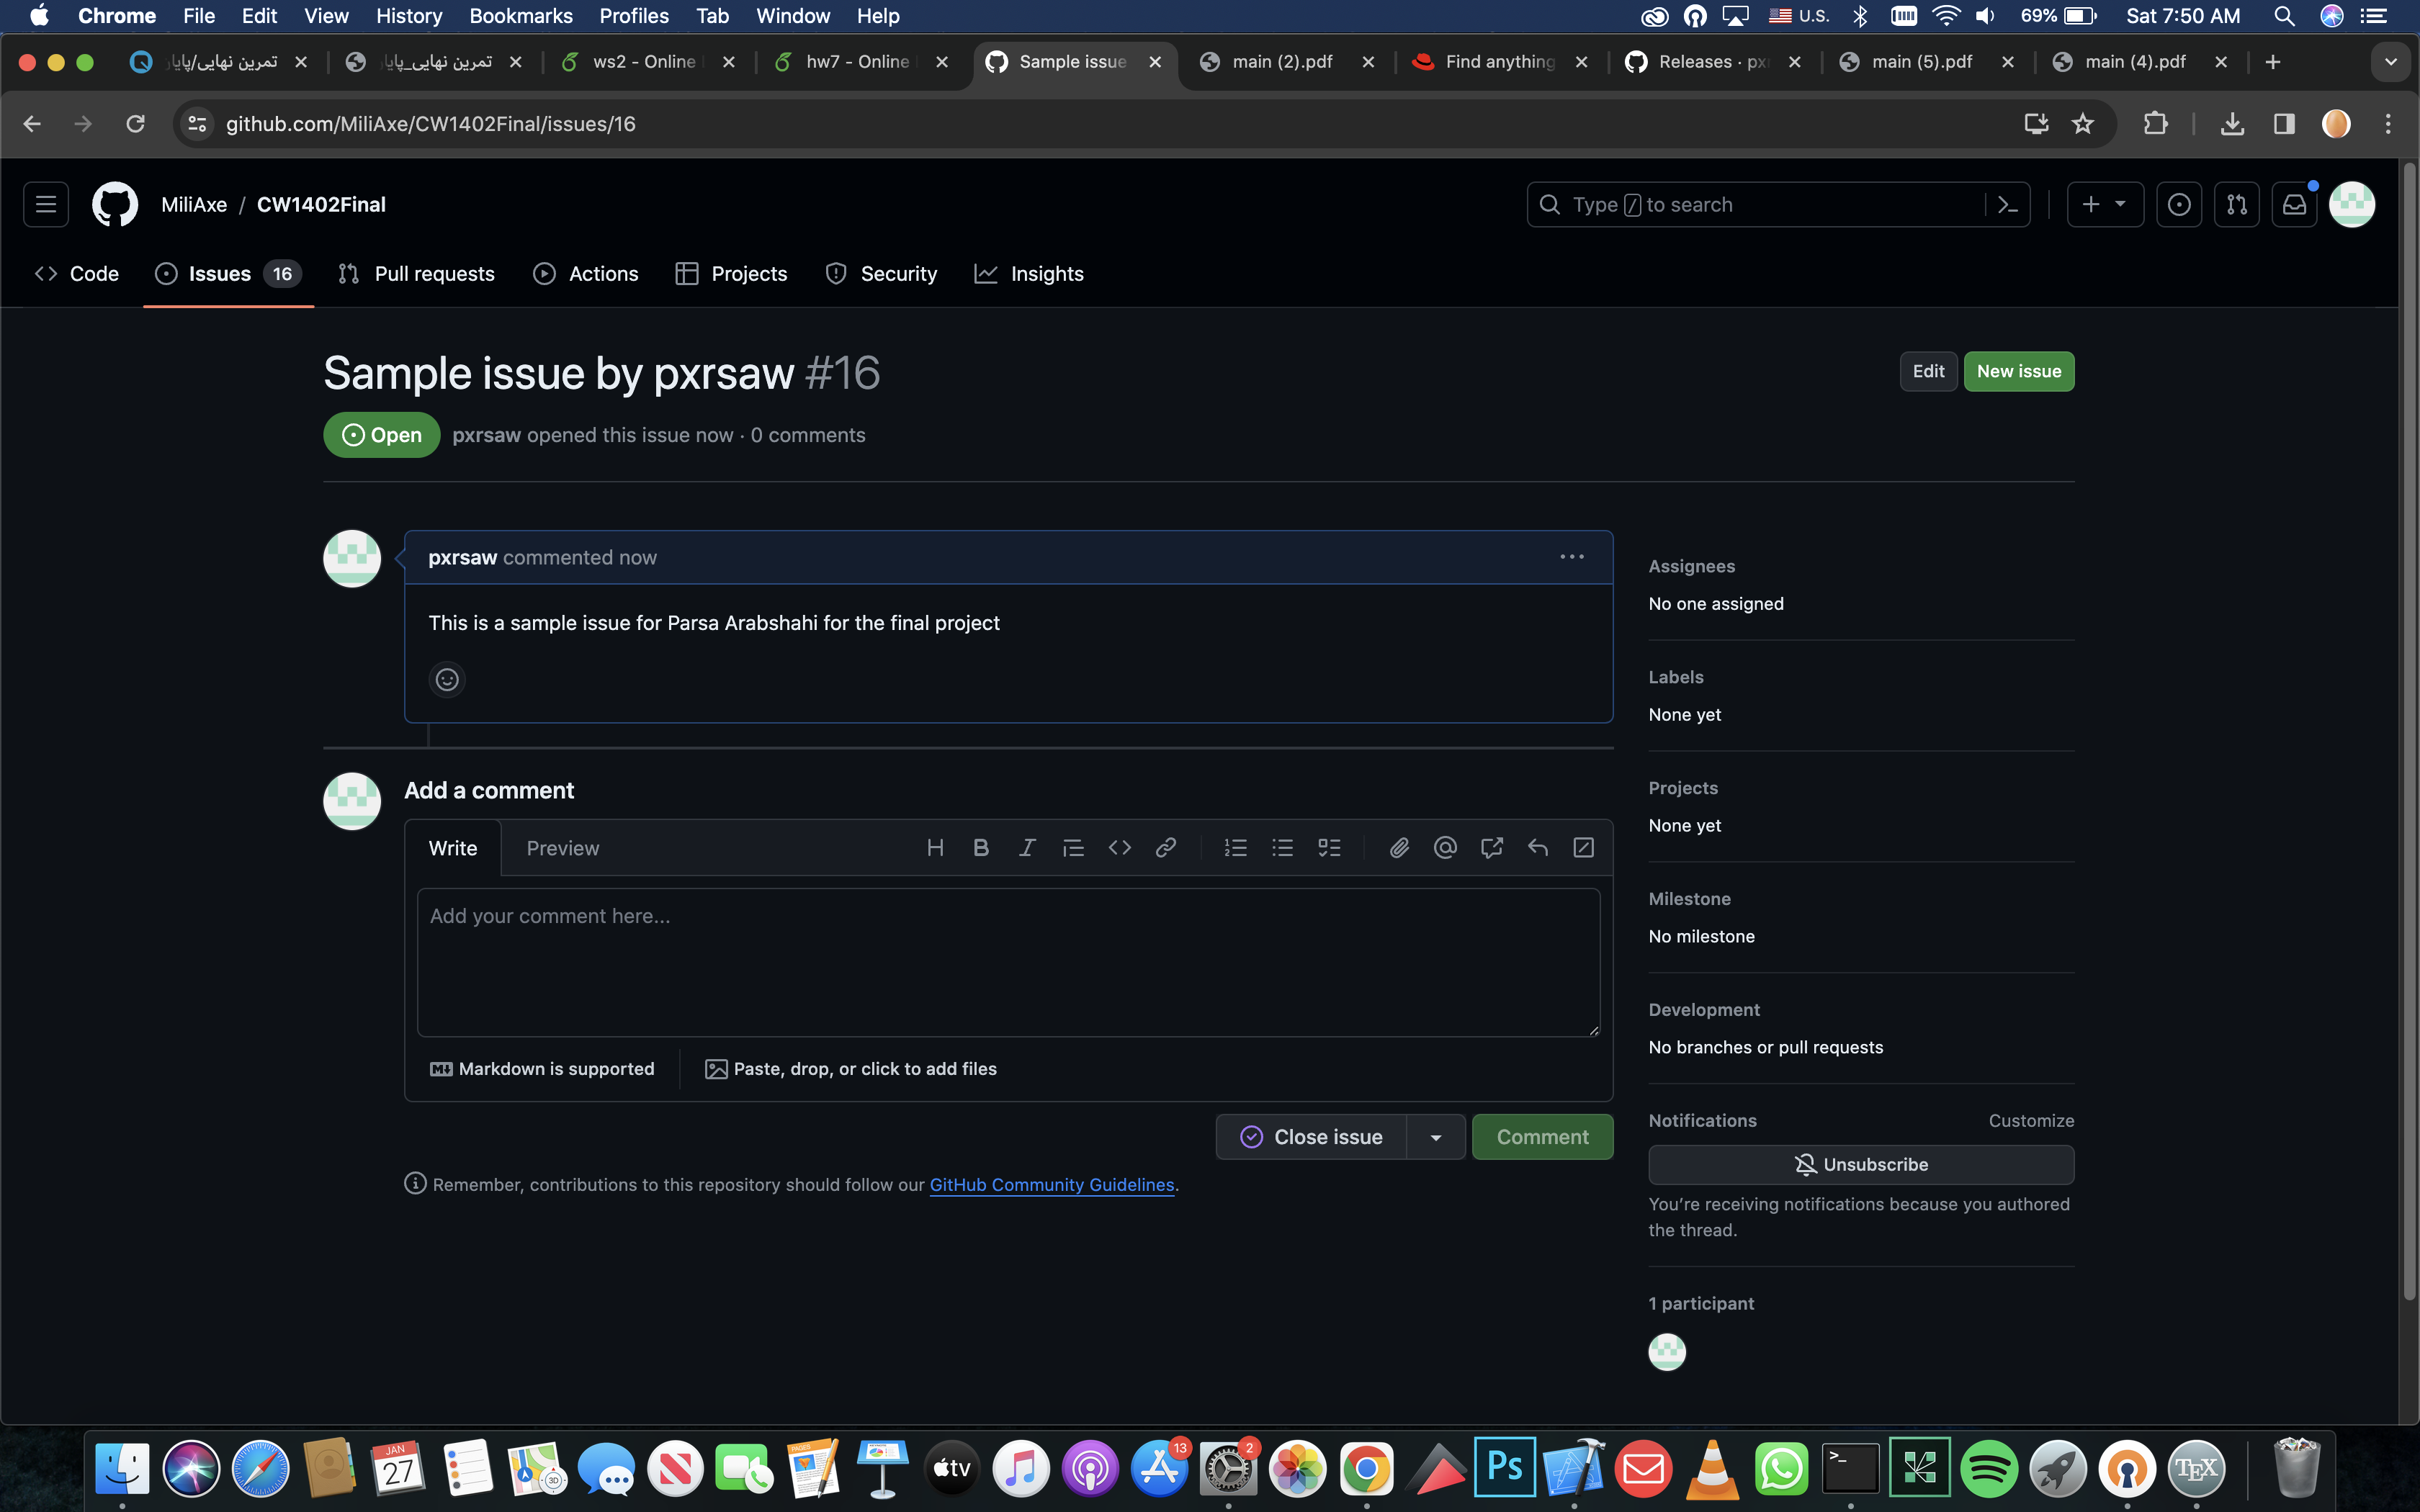
\includegraphics[width=0.7\textwidth]{finalproj.png}
\end{document}
